\documentclass[aspectratio=169]{beamer}

\usepackage[utf8]{inputenc}
\usepackage{array}
\usepackage{booktabs}
\usepackage{bold-extra}
\usepackage{graphics}
\usepackage{hyperref}
\hypersetup{%
  colorlinks=true,
  linkcolor=blue,
  filecolor=blue,
  urlcolor=cyan,
}
\usepackage{listings}
\usepackage{multicol}
\usepackage[absolute,overlay]{textpos}
\usepackage{setspace}
\usepackage{verbatim}
\usepackage{fancyvrb} % for verbatim centering
\usepackage{cancel}
\usepackage{ulem}
\usepackage{tikz}

\usetheme{Warsaw}
\usecolortheme{beaver}
\definecolor{clOrange}{HTML}{E76600}
\definecolor{clAlmostWhite}{HTML}{FEFFD9}
\definecolor{clGreen}{HTML}{007F00}
\definecolor{clFlag}{HTML}{D33682}
\definecolor{clFlagOpt}{HTML}{CB4B16}
\definecolor{clRedFlag}{HTML}{DC322F}
\definecolor{clViolet}{HTML}{4c0070}

\definecolor{clCodeBlue}{rgb}{0.0, 0.18, 0.38}
\definecolor{clCodeGreen}{rgb}{0.0, 0.27, 0.15}
\definecolor{clCodeRed}{rgb}{0.63, 0.0, 0.0}

\title[Friends09 ::The Rule Of ...]{The Rule of \xcancel{Big Three}\textsuperscript{\cancel{and a half}} \xcancel{Five} \cancel{Four\textsuperscript{and a half}} \xcancel{Seven} Zero\\
or\\
Evolution of Resource Management in C++ in the Recent Years
}
\author{Adam Graliński}
\date[FFFE\_21]{\textbf{C++ {\color{red}F}{\color{blue}F}{\color{green}F}{\color{yellow}E}, September 2021}}

\setbeamertemplate{navigation symbols}{}
\setbeamercolor{title}{fg=black}
\setbeamercolor{author}{fg=clAlmostWhite}
\setbeamercolor{date}{fg=clAlmostWhite}
\setbeamerfont{author}{size=\huge}
\setbeamerfont{date}{size=\Large}

\newcommand{\greenemph}[1]{\textit{\textcolor{clGreen}{#1}}}
\newcommand{\cppmethod}[1]{\texttt{\textbf{\textcolor{clCodeBlue}{#1}}}}

\lstset{
  language=C++,
  basicstyle=\ttfamily,
  keywordstyle=\color{clCodeBlue}\ttfamily,
  stringstyle=\color{clCodeGreen}\ttfamily,
  commentstyle=\color{clCodeRed}\ttfamily,
  morecomment=[l][\color{magenta}]{\#}
}

\begin{document}

{\usebackgroundtemplate{%
 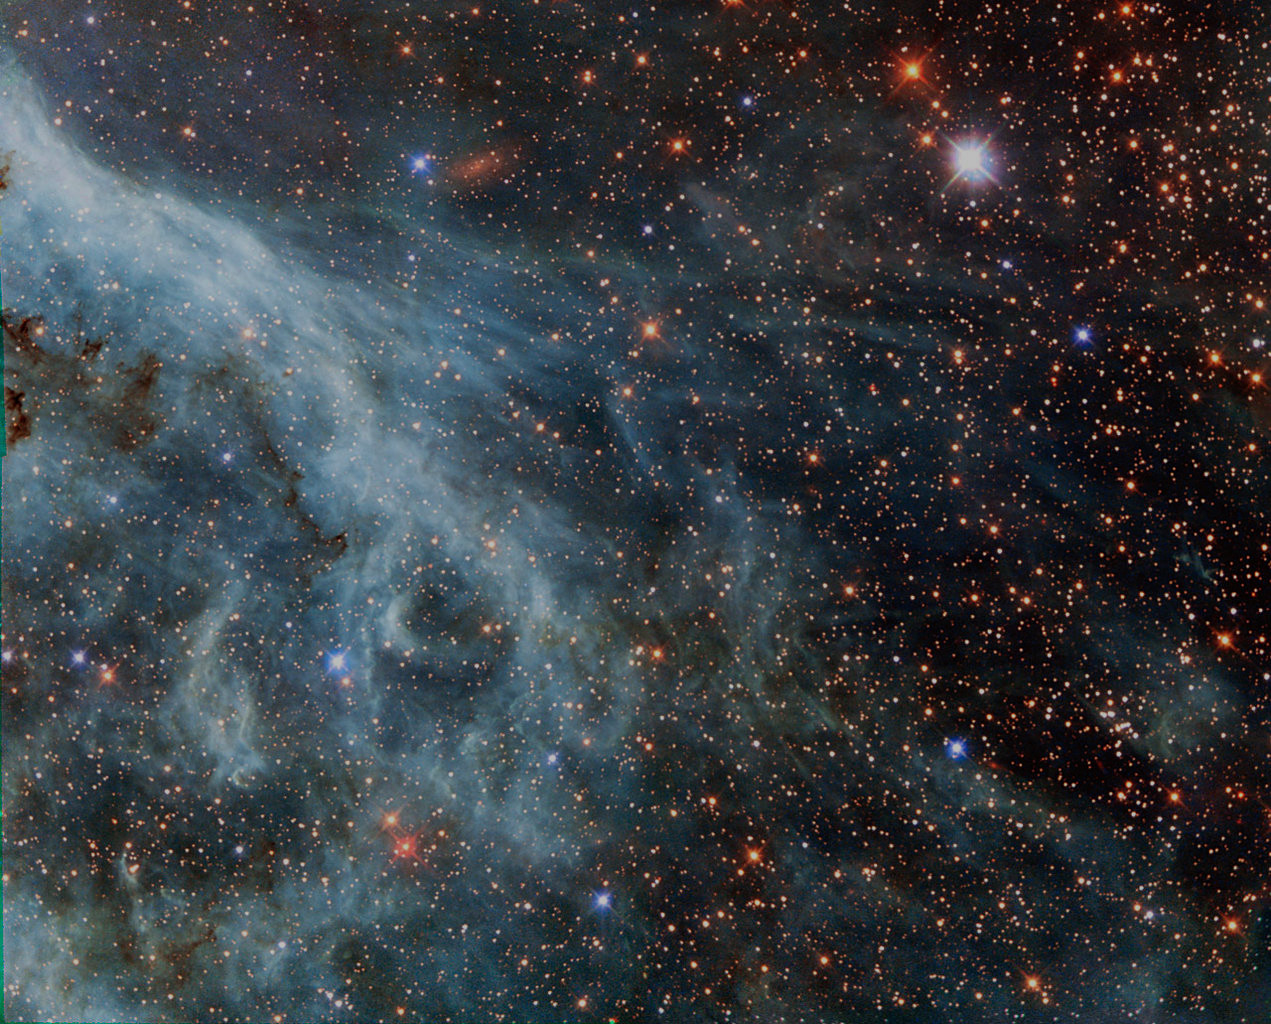
\includegraphics[width=\paperwidth,height=\paperheight]{../common/bg_galaxy.jpg}}
\begin{frame}
\titlepage{}
\end{frame}
}

\begin{frame}
\frametitle{Resource management}
\begin{itemize}
\item{Dynamic allocation and destruction of objects is, generally, hard.}
\item{do it wrong and spend hours debugging:}
\begin{itemize}
  \item{the \textcolor{clGreen}{crashes}, or}
  \item{the \textcolor{clOrange}{unexpected runtime behavior}}
\end{itemize}
\item{don't do it and just \textcolor{clRedFlag}{watch the memory leak}}
\end{itemize}
\vspace{1cm}
The first known solution there became known as the \greenemph{RAII} (or RRID) software pattern.
\end{frame}

\begin{frame}
\frametitle{RAII in the Dark Ages (C++98)}
\href{https://en.cppreference.com/w/cpp/language/raii}{en.cppreference.com/w/cpp/language/raii}
\begin{itemize}
  \item{encapsulate each resource into a class, where}
  \begin{itemize}
    \item{the constructor acquires the resource and establishes all class invariants or throws an exception if that cannot be done,}
    \item{the destructor releases the resource and never throws exceptions;}
  \end{itemize}
  \item{always use the resource via an instance of a RAII-class that either}
  \begin{itemize}
    \item{has automatic storage duration or temporary lifetime itself, or}
    \item{has lifetime that is bounded by the lifetime of an automatic or temporary object}
  \end{itemize}
\end{itemize}
Classes with open()/close(), lock()/unlock(), or init()/copyFrom()/destroy() member functions are typical examples of non-RAII classes.
\end{frame}

\begin{frame}
\frametitle{Problems with RAII}
This version of RAII just transfers the problems to the manager class.
\begin{itemize}
  \item{How to pass the resource around?}
  \item{Can the manager object be copied?}
\end{itemize}
The \greenemph{Rule of Big Three} was coined, and it was a good rule. For a while.\\
\vspace{0.5cm}
Meanwhile, the copy-and-swap idiom took traction.
\begin{itemize}
  \item{How to account for the copy-and-swap idiom?}
\end{itemize}
The Rule of Big Three became the Rule of Big Three\textsuperscript{\greenemph{and a half}}.
\end{frame}

\begin{frame}
\frametitle{The Rule of Big Three\textsuperscript{and a half}}
When writing a class that manages a dynamically-allocated resource, then:
\begin{enumerate}
\item{the resource may be passed-by-value (copied)}
\item{the resource may be assigned to another instance}
\item{the resource needs to be deallocated when falling out of scope}
\end{enumerate}
\vspace{0.1cm}
So, if you have implemented either:
\begin{enumerate}
\item{a copy constructor}
\item{an assignment operator}
\item{a destructor}
\end{enumerate}
then you need to implement \greenemph{all three of them}.\\
\vspace{0.5cm}
\greenemph{\textsuperscript{and a half}}: also implement own \texttt{swap()} function for copy-and-swap idiom.
\end{frame}

\begin{frame}
\frametitle{The Rule of Big Three --- a simple example}
{\fontsize{8}{6} \lstinputlisting{code/Person.cpp}}

\end{frame}

\begin{frame}
\frametitle{The Rule of Big Three --- a simple example}
\begin{columns}
  \begin{column}{0.45\textwidth}
    {\fontsize{4}{4} \lstinputlisting{code/Person.cpp}}
  \end{column}
  \begin{column}{0.55\textwidth}
    {\fontsize{4}{4} \lstinputlisting{code/rule3.cpp}}
  \end{column}
\end{columns}
\end{frame}

\begin{frame}
\frametitle{C++11: Move Semantics}
C++11 is a game changer. With its concept of the \textit{r-value reference} one can finally force to \textbf{move} where C++98 would \textbf{copy}.
\\
\vspace{1cm}
The resource managing classes now must also account for move semantics - the \textbf{move constructor} and \textbf{move assignment operator}.
\end{frame}

\begin{frame}
\frametitle{The Rule of Big Five --- a simple example}
\begin{multicols}{2}
  {\fontsize{4}{4} \lstinputlisting{code/rule5.cpp}}
\end{multicols}
\end{frame}

\begin{frame}
\frametitle{The Rule of Big Four\textsuperscript{and a half}}
If you have implemented either:
\begin{enumerate}
\item{the copy constructor}
\item{the assignment operator}
\item{the move constructor}
\item{the swap function}
\end{enumerate}
then you need to \xcancel{implement} \greenemph{define the usage} of all of them.
\end{frame}

\begin{frame}
\frametitle{The Rule of Zero}
There is an alternative to \textcolor{clViolet}{The Rule of Big Four\textsuperscript{and a half}}, called \greenemph{the Rule of Zero}:\\
\begin{center}
\textbf{You should \emph{never} implement a destructor, copy constructor,\\move constructor or assignment operators}.
\end{center}
With one important corollary rule:
\begin{center}
\textbf{You should \emph{never} manage a resource via a raw pointer}.
\end{center}
\vspace{1cm}
...but what if you \emph{must} create object dynamically?
\end{frame}

\begin{frame}
\frametitle{If you must create objects dynamically...}
Use \texttt{std::unique\_ptr} or \texttt{std::shared\_ptr}
\begin{itemize}
\item{\texttt{std::unique\_ptr} for resources that can be \textcolor{clGreen}{moved}, but not \textcolor{clRedFlag}{copied}}
\item{\texttt{std::shared\_ptr} for resources that can be both \textcolor{clGreen}{moved} and \textcolor{clGreen}{copied}}
\end{itemize}
\end{frame}

\begin{frame}
\frametitle{Rule of Zero --- really simple example}
  {\fontsize{4}{4} \lstinputlisting{code/rule0.cpp}}
\end{frame}


\begin{frame}
\frametitle{Key takeaways}
{\centering
\begin{itemize}
  \item Don't make your life unnecessary hard
  \item Let the standard library take care of your objects' lifetime
  \item Use smart pointers wherever you can
\end{itemize}

\vspace{2ex}
\begin{center}{\Large Thank you!}\end{center}
}
\end{frame}

\end{document}
